\documentclass[conference]{IEEEtran}
\usepackage[utf8]{inputenc}
\usepackage[T1]{fontenc}
\usepackage{listings}
\usepackage{amsmath}



%Portuguese-specific commands
%--------------------------------------
\usepackage[portuguese]{babel}
%--------------------------------------
\usepackage{hyphenat}
\hyphenation{mate-mática recu-perar}

\usepackage{array}
\newcolumntype{L}[1]{>{\raggedright\let\newline\\\arraybackslash\hspace{0pt}}m{#1}}
\newcolumntype{C}[1]{>{\centering\let\newline\\\arraybackslash\hspace{0pt}}m{#1}}
\newcolumntype{R}[1]{>{\raggedleft\let\newline\\\arraybackslash\hspace{0pt}}m{#1}}


\ifCLASSINFOpdf   
   \usepackage[pdftex]{graphicx}     
   % declare the path(s) where your graphic files are       
   \graphicspath{{../pdf/}{../jpeg/}{./image/}}    
   % and their extensions so you won't have to specify these with    
   % every instance of \includegraphics      
   \DeclareGraphicsExtensions{.pdf,.jpeg,.png,.jpg}   
 \else   
   % or other class option (dvipsone, dvipdf, if not using dvips). graphicx     
   % will default to the driver specified in the system graphics.cfg if no   % driver is specified.    
   \usepackage[dvips]{graphicx}   
   % declare the path(s) where your graphic files are     
   \graphicspath{{../eps/}}    
  % and their extensions so you won't have to specify these with   
  % every instance of \includegraphics    
  % \DeclareGraphicsExtensions{.eps}   
\fi
\usepackage{graphicx}


% correct bad hyphenation here

\begin{document}
\title{Aplicação do Modelo SIR-Vetorial para Modelagem da Dengue no Brasil}

\author{
\IEEEauthorblockN{
Bruno Ponciano Marques,
Gabriel Barbosa Candido,
Igor Correa Nunes e
Luis Felipe Mileo Sant ana\IEEEauthorrefmark{4}}
\IEEEauthorblockA{
Universidade Federal de Itajubá Itajubá - Minas Gerais - Brasil\\ Email: 
bruno.ponciano1999@gmail.com,
gabcandido98@gmail.com,
igorconunes@gmail.com,
mileo@unifei.edu.br
}}

%EU ACHEI MUITO MELHOR, SÓ COLOQUEI O ANEXO DEPOIS DA REFERÊNCIA. A INTRODUÇÃO AINDA ESTA GRANDE, MAS ESTA BOM. EU SO MELHORIA O PLOT. SE IMPRIMIR ELE VAI CONSEGUIR LER A LEGENDA????


%O TEXTO AGORA ESTA BEM ESTRUURADO, ACHO QUE ELE VAI GOSTAR MUITO.

%TAMBÉM ACHO QUE PODEMOS MELHORAR UM POUCO E PASSAR PARA INGLES, SUBMETER PARA ALGUM JOURNAL DE MODELAGEM. É UMA BOA APLICAÇÃO
\maketitle

\begin{abstract}
%\boldmath
Dengue is an endemic disease that regularly appears in Brazil, more precisely in hot periods and infects thousands because it is easily transmitted. However, scientific research in the field of modeling and analysis of dynamic systems grows considerably. t was verified the existence of many mathematical models for modeling and analysis of Dengue, using some especific parameters, such as infected persons and the growth rate of the disease vector. Therefore, in qualitative analysis, it is to evaluate the SIR-VECTOR mathematical model presented for the adaptation of this one with data referring to the Brazilian reality to analyze dengue in Brazil and/or in each state of the country in a more precise way.

Key words: Modeling of dynamic systems, SIR-VECTOR Model for Dengue, Analysis of Dengue in Brazil, Python.
\end{abstract}


\IEEEpeerreviewmaketitle

\section{Introdução}

A dengue é uma doença endêmica vetorial, reconhecida como a maior arbovirose do mundo com mais de 50 milhões de casos por ano\cite{10.1371/journal.pone.0049085}. No Brasil, em 2008, a incidência da doença alcançou aproximadamente 800
casos por 100 mil habitantes\cite{bohm2016dengue}. Nos últimos anos diversos estudos foram realizados para compreender o comportamento desta endemia. Realizados de forma analítica através de modelos matemáticos diversos\cite{kermack1927contribution,bailey1975mathematical,daley2001epidemic,brauer2001mathematical,nishiura2006mathematical,10.1371/journal.pone.0049085}. Realizou-se um estudo a estes modelos matemáticos e elaborou-se simulações computacionais comparativas para empoderar os interessados em entender, determinar e prevenir as causas da Dengue.


\subsubsection{Doenças Endêmicas no Brasil}

 Endemia é uma enfermidade, geralmente infecciosa que reina constantemente certo país ou região por influência de causa local \cite{brasil2001controle6}.
	As principais doenças endêmicas do Brasil são: a malária; a leishmaniose; a esquistossomose; a febre amarela; a dengue;  o tracoma; a doença de Chagas; a Hanseníase; a tuberculose; a cólera e a gripe A.
Um dos maiores desafios à saúde pública atualmente são grandes endemias, uma vez que atingem principalmente pessoas menos favorecidas, entre as doenças endêmicas citadas a maioria delas são oriundas da pobreza, isto é, de condições precárias de vida, a falta de saneamento básico é um dos principais fatores que contribuem para o aparecimento de algumas doenças, tais como: a malária, a cólera, a hanseníase, etc.
\subsubsection{Dengue}
A dengue é uma doença infecciosa febril aguda causada por um vírus da família flaviviridae e é transmitido ao homem através do mosquito Aedes aegypti, também infectado pelo vírus. Atualmente a dengue é considerada um dos principais problemas de saúde pública de todo o mundo. Existem quatro sorotipos de dengue em todo o mundo: DEN-1, DEN-2, DEN-3  e DEN-4.\\
% verificar se esta citação esta correta
\indent Segundo a publicação da Revista da Sociedade Brasileira de Medicina Tropical\cite{penna2008influence} a dengue apresenta uma das grandes preocupações do Ministério da saúde, devido à quantidade de casos notificados todos os anos. Por abranger quase a totalidade do território nacional, há risco potencial de ocorrer novas epidemias associadas à circulação do sorotipo DEN-3 e a possibilidade da entrada do DEN-4, único sorotipo que ainda não tem disseminação no país.
A dengue é hoje uma das doenças com maior incidência no Brasil, atingindo a população de todos os estados, independentemente da classe social.\\
\indent Tauil \cite{tauil2002critical} afirma que a dengue é hoje a arbovirose mais importante do mundo. Cerca de 2,5 bilhões de pessoas encontram-se sob risco de se infectarem, particularmente em países tropicais onde a temperatura e a umidade favorecem a proliferação do mosquito vetor. Entre as doenças re-emergentes é a que se constitui em problema mais grave de saúde pública. São bem conhecidas sua etilogia e seus mecanismos de transmissão. O seu espectro clínico é muito amplo, variando de formas assintomáticas ou oligossintomáticas até formas graves  e letais. A dengue pode se apresentar clinicamente em quatro formas diferentes são elas: Infecção inaparente, Dengue clássica, Febre hemorrágica da dengue e Síndrome de choque da dengue.\\
\indent Os tipos de dengue que mais se destacam é a Dengue Clássica e a Hemorrágica. A dengue clássica é semelhante a gripe, é uma das formas mais leve da doença. A pessoa quando infectada tem febre alta entre 39ºC e 40ºC, forte dor de cabeça dor atrás do olhos, que piora com o movimento dos mesmos, perda do paladar e apetite, manchas e erupções na pele semelhantes ao sarampo, principalmente no tórax e membros superiores, náuseas e vômitos, tonturas, extremo cansaço, moleza, dor no corpo e muitas dores nos ossos e articulações. A dengue hemorrágica é uma forma grave da doença, quando a pessoa é infectada pela segunda vez. No início os sintomas são iguais ao dengue clássico, mas após o 5º dia da doença, alguns pacientes começam a apresentar sangramento e choque.\\
\indent Os sangramentos ocorrem em vários órgãos. Alguns doentes apresentam choque circulatório. Esse tipo de dengue pode levar a pessoa ao óbito. Os principais sintomas da dengue hemorrágica são:
\begin{itemize}
    \item Dores abdominais fortes e contínuas;
    \item Pele  pálida fria e úmida;
    \item Vômitos persistentes;
    \item Sangramento pelo nariz, boca e gengivas;
    \item Manchas vermelhas na pele;
    \item Sonolência, agitação e confusão mental;
    \item Sede excessiva e boca seca;
    \item Pulso rápido e fraco;
    \item Dificuldade respiratória;
    \item Perda de consciência;
\end{itemize}

\indent O Ministério da Saúde \cite{brasil2002} afirma que para os casos da dengue clássica, não há tratamento específico. A medicação é apenas sintomática com analgésicos e antitérmicos (paracetamol e dipirona). Devem ser evitados os salicilatos e os anti-inflamatórios não hormonais, já que seu uso pode favorecer o aparecimento de manifestações hemorrágicas e acidose. O paciente deve ser orientado a permanecer em repouso e iniciar hidratação oral. \\

% \indent Para a prevenção da dengue é necessário a eliminação do criadouro de larvas do Aedes Aegypti, para isso podemos tomar medidas como:
% \begin{itemize}
%     \item Substituir a água dos vasos de plantas por terra e manter seco o prato coletor de água.
%     \item Desobstruir as calhas do telhado, para não haver acúmulo de água.
%     \item Não deixar pneus ou qualquer recipiente que possa acumular água expostos à chuva.
%     \item Manter sempre tampadas as caixas d’água, cisternas, barris e filtros.
%     \item Acondicionar o lixo em saco plástico fechado ou latões com tampa.\\
% \end{itemize}

\subsubsection{Vacina}
A vacina contra dengue no Brasil foi aprovada pela Anvisa em dezembro de 2015, porém não é oferecia pelo Programa Nacional de Imunizações(PNI) sendo assim disponível somente na rede privada. \\ 
A empresa francesa Sanofi-Aventis é, até o momento, a única empresa, no país, com registro de uma vacina contra a dengue, chamada de Dengvaxia®. O tratamento com a vacina inclui três doses, com seis meses de intervalo entre elas. Outras vacinas para a prevenção da dengue ainda estão sendo analisadas pela Anvisa, para que possam ser comercializadas no Brasil com segurança e eficácia. Cada dose da vacina custa de 130 à 140 reais(variando de acordo com o estado) para uso pediátrico ou adulto (pessoas de 9 a 45 anos).
\indent O produto é indicado para imunização contra os 4 (quatro) subtipos do vírus da dengue.
Posteriormente em 2018 a empresa que produz a vacina divulgou que ela é indicada para pessoas soropositivas (já contraíram a doença alguma vez) \cite{anvisa}.
Devido ao valor e a maior incidência de casos de contaminação ocorrer em regiões carentes, o número de vacinas não será relevante na modelagem.\\

\subsection{Modelagem de Sistemas Dinâmicos}
Segundo \cite{zambroni} ``Modelar um sistema físico qualquer significa obter uma representação matemática que permita um estudo analítico coerente com o comportamento do sistema na prática. 
Assim, os resultados obtidos devem representar, da maneira mais fidedigna possível, o sistema físico analisado. 
A fase de modelagem é vital, uma vez que o compromisso entre precisão e complexidade do modelo em relação à dificuldade de obtenção da resposta deve ser assumido. A complexidade de se modelar um sistema dinâmico depende fundamentalmente do conhecimento que se tem desse sistema.`` \\
	A metodologia adotada foi divida em três etapas descritas abaixo:
\begin{enumerate}
    \item Modelagem: Descrita anteriormente, consiste em representar o sistema físico através de um modelo matemático.
    \item Determinação das características dinâmicas: Implica em um levantamento prévio de dados, já que propriedades intrínsecas do sistema são consideradas.
    \item Análise: Consiste em, através de uma metodologia qualquer, analisar a resposta do sistema a uma entrada, excitação ou distúrbio.
\end{enumerate}
A figura \ref{fig:processo} mostra um fluxograma das etapas necessárias para o processo de modelagem:

\begin{figure}[!ht]
  \caption{Processo de modelagem de um sistema dinâmico}
  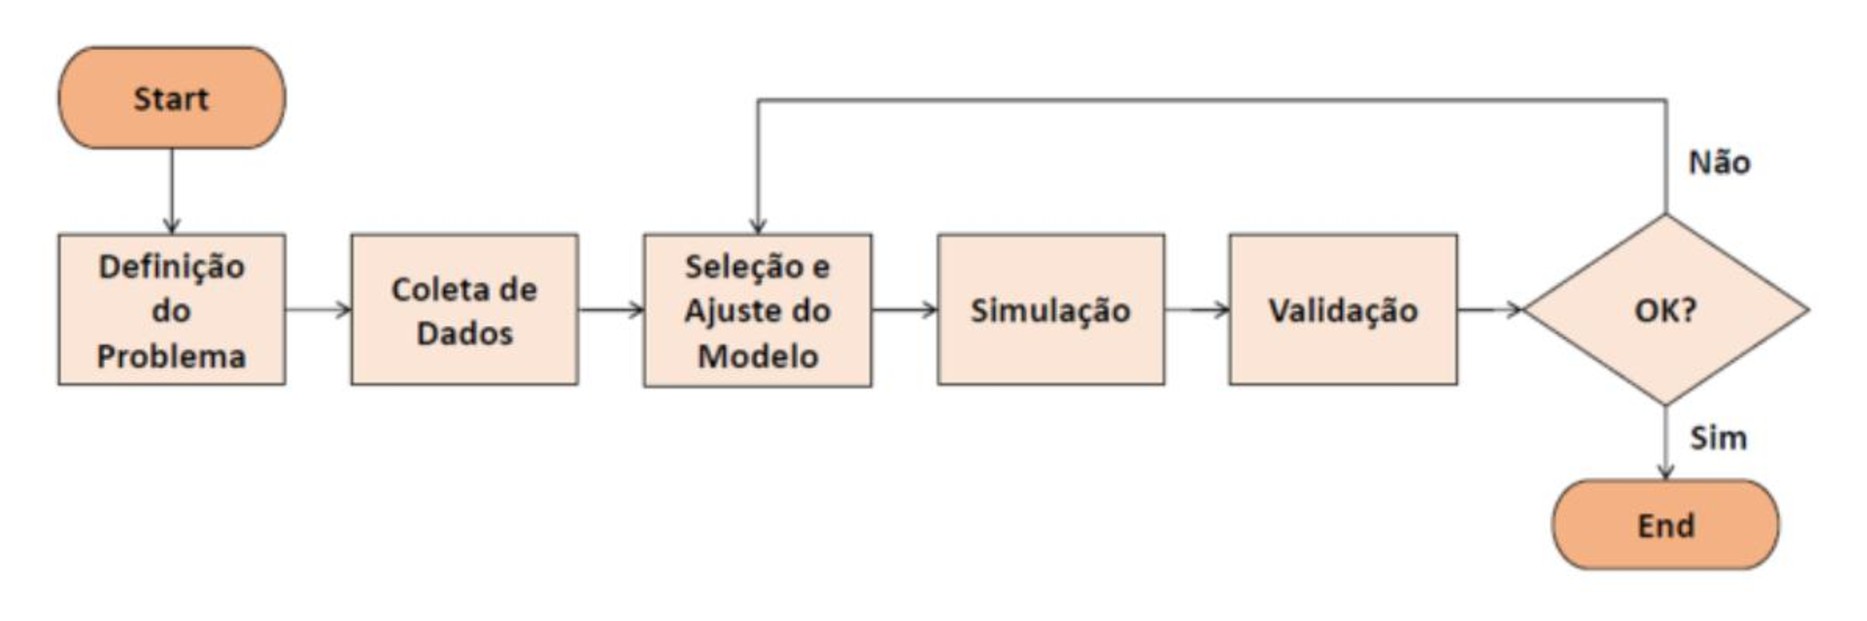
\includegraphics[width=0.5\textwidth]{workflow.eps}
  \label{fig:processo}
\end{figure}

Para o início do estudo foi definido um tema geral, as doenças endêmicas. A fim de uma abordagem mais específica e concreta, refinou-se o tema até a Dengue. A hipótese/tese do estudo foi:
	Estabelecer analise e comparações por meios analíticos a respeito de dados da Dengue, tendo em base como épocas de epidemia, regiões mais suscetíveis ao espalhamento do patógeno e seus hospedeiros primários do vírus. O estudo também teve seu foco em aplicar certo modelo matemático para prever os casos da doença em anos futuros tal como comprovar a eficácia do modelo adaptando-o para a realidade brasileira.
    	Em posse do objetivo principal e utilizando de diversos estudos prévios, foi realizada a coleta de dados para uma correta e realística aplicação do modelo. Após a determinação de alguns parâmetros que modelam e descrevem o sistema de espalhamento de doenças, foram analisados aqueles que têm maior importância nesse sistema e assim prosseguir para o processamento e análise dos resultados.

\subsubsection{Modelo SIR}
Nesta seção, procura-se ilustrar, através de um modelo simples (SIR), como a Matemática pode ser útil na previsão da evolução de uma epidemia e na tomada de decisão sobre estratégias de combate à sua propagação (vacinação, quarentenas, etc.).

Em 1927, \cite{kermack1927contribution} criaram um modelo em que se considera uma população fixa com apenas três compartimentos: sensíveis, S(t); infectado, I(t), e removido, R(t). Os compartimentos utilizados para este modelo consistem em três classes:\\
\begin{enumerate}
    \item S(t) é usado para representar o número de indivíduos não infectados com a doença no momento t, ou aqueles suscetíveis à doença.
    \item I(t) representa o número de indivíduos que tenham sido infectadas com a doença e que são capazes de transmitir a doença aos da categoria susceptível.
    \item R(t) é o compartimento utilizado para aqueles indivíduos que foram infectados e, de seguida, removidos a partir da doença, quer devido à imunização ou devido à morte. Os que estão nesta categoria não são capazes de ser infectados novamente ou para transmitir a infecção a outras pessoas.
\end{enumerate}
	O fluxo do presente modelo pode ser considerado da seguinte forma
	\begin{equation}
	    S - I - R
	\end{equation}

	Usando uma população fixa, 
	\begin{equation}
	    N=S(t)+I(t)+R(t)
	\end{equation}, Kermack e McKendrick derivadas das seguintes equações:
	
\begin{align}
    \frac{dS}{dt} &= -\beta SI\\
    \frac{dI}{dt} &= \beta SI - \gamma I\\
    \frac{dR}{dt} &= \gamma I
\end{align}

	 Foram feitas algumas hipóteses na formulação destas equações: em primeiro lugar, um indivíduo na população deve ser considerado como tendo uma probabilidade igual a todos os outros indivíduos de contrair a doença, com uma taxa de $\beta$, que é considerada a velocidade de infecção da doença. Portanto, um indivíduo infectado entra em contato e é capaz de transmitir a doença a outros $\beta$N por unidade de tempo e a fração de contatos por uma pessoa infectada com um susceptíveis é $\frac{S}{N}$. 
	O número de novas infeções na unidade de tempo por infecciosa é, então, $\beta$N$\frac{S}{N}$, dando a taxa de novas infeções (ou aqueles que deixam a categoria suscetível) como \cite{brauer2001mathematical}:
	
	\begin{equation}
	\beta \frac{S}{N}I = \beta SI
	\end{equation}
	
	  Para a segunda e terceira equações, considerar a população deixando a classe suscetível como sendo igual ao número de entrar na classe infectado. 
	No entanto, um número igual à fração ($\gamma$ , que representa a taxa de recuperação média/morte, ou $1/\gamma1$/ o período infeccioso médio) de infecciosos estão a deixar esta classe por unidade de tempo para entrar na classe removida. Estes processos que ocorrem simultaneamente são referidos como a Lei da Ação de Massa, uma ideia amplamente aceite de que a taxa de contágio entre dois grupos numa população é proporcional ao tamanho de cada um dos grupos envolvidos \cite{daley2001epidemic}.

\subsubsection{O modelo SIR com nascimentos e mortes}
Usando o processo do sarampo, por exemplo, existe uma chegada de novos indivíduos suscetíveis na população. Para este tipo de situação nascimentos e mortes devem ser incluídas no modelo. As seguintes equações diferenciais representam este modelo, assumindo uma taxa de mortalidade u e taxa de natalidade igual à taxa de mortalidade:

\begin{align}
\begin{split}
    \frac{dS}{dt} &= -\beta SI + u(N-S)\\
    \frac{dI}{dt} &= \beta SI- \gamma I - uI\\   
    \frac{dR}{dt} &= \gamma I - uR
\end{split}
\end{align}\\

\subsubsection{Modelo SIR Vetorial}
Em 1975 por Bailey\cite{bailey1975mathematical} propôs uma forma simples de modelar uma endemia, que depende de um vetor para se propagar. Correspondendo a base de nossa simulação, que explora os detalhes do boletim de Hiroshi \cite{nishiura2006mathematical} e o abrangente detalhamento realizado posteriormente  no periódico\cite{10.1371/journal.pone.0049085}.

\begin{figure}[!ht]
  \caption{Modelo de interação entre populações humanas e de vetores}
  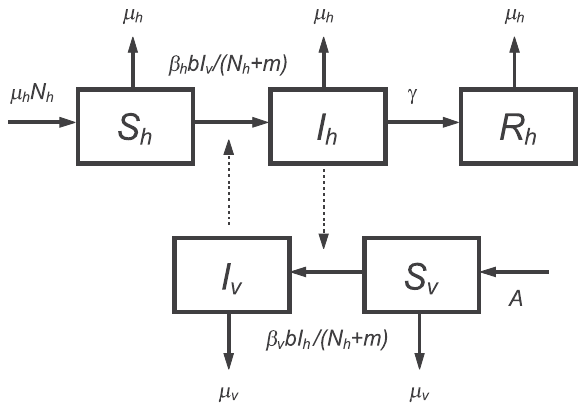
\includegraphics[width=0.46\textwidth]{modelosirvetorial.png}
    \label{fig:modelo}
\end{figure}

Reapresentado na figura \ref{fig:modelo} e no conjunto de equações \ref{ref:equacoesvector}.

\begin{align} \label{ref:equacoesvector}
\begin{split}
    \frac{dSh}{dt} &= uh (Nh - Sh) - \frac{\beta h* b}{Nh + m} Sh * Iv\\
    \frac{dIh}{dt} &= \frac{\beta h * b}{Nh + m} Sh * Iv - (uh + \gamma)Ih\\
    \frac{dRh}{dt} &=  \gamma Ih - uh*Rh\\
    \frac{dSv}{dt} &= A - \frac{\beta v* b}{Nh + m} Sv * Ih - uv*Sv\\
    \frac{dIv}{dt} &=  \frac{\beta v * b}{Nh + m} Sv * Ih - uv*Iv
\end{split}
\end{align}\\

A abordagens matemática,nos permite examinar a condição de limite e determinar a estabilidade local ou global através de experimentos analíticos. Além disso, também é possível examinar o impacto de várias estratégias de intervenção (por exemplo, controle de vetores) na progressão epidêmica em uma população hipotética, estendendo os pressupostos extrínsecos das equações \ref{ref:equacoesvector}\cite{nishiura2006mathematical}.

\section{Desenvolvimento}

Visando realizar a aplicação prática do modelo definido no item anterior, desenvolveu-se algorítimos para realizar a simulação computacional do conjunto de equações \ref{ref:equacoesvector}. O algorítimo pode ser visto em detalhes no ANEXO I e/ou referência externa \cite{mileo}. Além disso realizou-se o levantamento dos parâmetros de entrada descritos a seguir.

\subsection{Parâmetros considerados}

\subsubsection{Parâmetros explícitos}
Os parâmetros explícitos (os que são variáveis pelo usuário no momento da análise e são mostrados no gráfico do modelo matemático) foram definidos na tabela \ref{table:1}.

\begin{table}[!ht]
\begin{tabular}{| c | L{5cm} | c |}
Parâmetro & Descrição & Fonte\\
 \hline\hline
 Nh & População da amostra  & Fixo \\ \hline
 A & Taxa constante de novos mosquitos que entram na população & \cite{10.1371/journal.pone.0049085} \\ \hline
 $\mu $v & Mortalidade per capita dos mosquitos & \cite{10.1371/journal.pone.0049085} \\ \hline
\end{tabular}
\caption{Parâmetros explícitos}
\label{table:1}
\end{table}

\subsubsection{Parâmetros implícitos} 

Os parâmetros implícitos (isto é, que existem nos cálculos e no desenvolvimento do modelo mas não estão aparentes no momento da simulação) que foram considerados para esse modelo matemático foram definidos na tabela \ref{table:2}.

\begin{table}[!ht]
\begin{tabular}{| c | L{5cm} | c |}
Parâmetro & Descrição & Fonte\\
 \hline\hline
 $ \beta $h & Probabilidade de transmissão do Vetor - Humanos & \cite{nishiura2006mathematical,10.1371/journal.pone.0049085} \\ \hline
 $ \gamma $ & Taxa de humanos infectados que se recuperam e ficam imunes a doença & \cite{espiritosanto} \\ \hline
 $\mu $h & Taxa per-capita de mortalidade dos humanos não relacionado a doença & \cite{ibge-mortalidade} \\ \hline
 b & Quantas vezes por dia um mosquito morde as pessoas & \cite{10.1371/journal.pone.0049085} \\ \hline
 m & Número dos hospedeiros alternativos & \cite{nishiura2006mathematical} \\ \hline
 $ \beta $v & Probabilidade de transmissão Humano - Vetor & \cite{10.1371/journal.pone.0049085} \\ \hline
 Ih & Número de indivíduos infectados quando o modelo começou a rodar & \cite{svs} \\ \hline
 Rh & Número de indivíduos recuperados no inicio da execução do modelo & \cite{svs} \\ \hline
 Sv & O número de vetores suscetíveis no início da execução do modelo & Não Aplicável \\ \hline
 Iv & O número de vetores infectados no início da execução do modelo & Não Aplicável \\ \hline
 Sh &  Número dos humanos suscetíveis no inicio do modelo & Não Aplicável \\ \hline
 t & tempo de simulação (dias)  & * \\ \hline
\end{tabular}

\caption{Parâmetros implícitos \protect\\ * - Definido experimentalmente conforme a estabilidade do sistema}
\label{table:2}
\end{table}

O vetor de condições iniciais é tal que: 
  $$
  y0 = \left[
\begin{array}{rrrrr}
 Sh & Ih & Rh & Sv & Iv
\end{array}\right]
$$

\section{Análise de Resultados}

Para iniciar a simulação, considerou-se os seguintes valores para cada parâmetro implícito:\\

$ \beta h $ = 0.75 ;

$
 \gamma$ = 0.25 ;
 
$
uh $ = 6/1000 ;

$b$ = 1;

$ m$ = 0;

$ \beta v$ = 1;

$ Ih $ = 49.2 ;

$Rh$ = 49.2 ;

$Sv$ = 0 ;

$Iv$ = 0;
 
$Sh$= Nh - Ih ;\\

Foram realizadas dez simulações com o modelo matemático para a análise dos resultados. Ao longo destas simulações, variou-se os parâmetros explícitos conforme o produto das matrizes:\\

\begin{itemize}
    \item Nh - População da amostra, se manteve um número constante, mantendo a proporção com a população de infectados\cite{svs}; [100.000]
    \item A  - Taxa constante de novos mosquitos que entram na população; [400, 800, 1600, 3200, 5000]
    \item uv - Mortalidade per capita dos mosquitos. [0.1,  0.25]
\end{itemize}

Uma discussão breve será levantada após cada simulação e posteriormente uma análise geral sobre todas as simulações com maior aprofundamento nos parâmetros utilizados. Desta forma, o intuito é variar a relação entre a densidade de mosquitos e a população de seres humanos. \\[0.15 cm]

\subsubsection{Simulação 1: A 400 - uv 0.1}

Pode-se observar na figura \ref{fig:s1} que com os parâmetros atuais, a taxa de proporção de infectados é mínima, ou seja, não há contágio da doença. Uma das possibilidades de justificativa a discutir é devido a densidade de vetores da doença ser muito inferior à população, desta forma, não se tem proliferação suficiente para um surto endêmico.\\

\begin{figure}[!ht]
  \caption{Simulação 1 - Nh 100000 - A 400 - uv 0.1}
  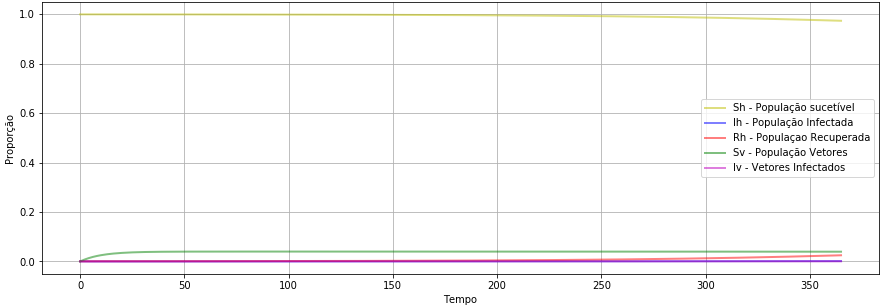
\includegraphics[width=0.46\textwidth]{Graf1.png}
  \label{fig:s1}
\end{figure}

\subsubsection{Simulação 2: A 400 - uv 2.50}

Nesta simulação, figura \ref{fig:s2}, em comparação com a simulação anterior, aumentou-se a taxa de mortalidade dos vetores, consequentemente, o modelo matemático mostra uma diminuição na proporção da população dos vetores o que é logicamente viável devido ao aumento da mortalidade
\\

\begin{figure}[!ht]
  \caption{Simulação 2 - Nh 100000 - A 400 - uv 2.50}
  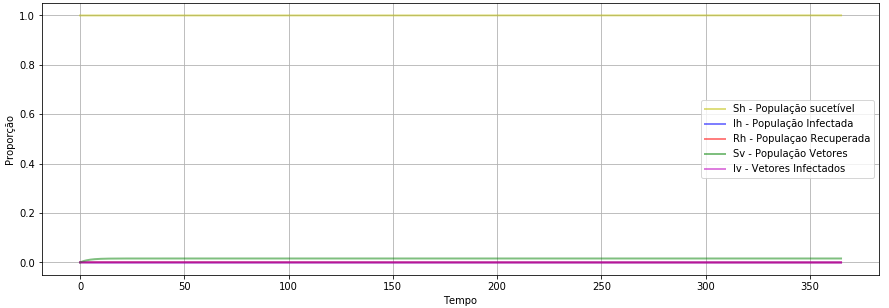
\includegraphics[width=0.46\textwidth]{Graf2.png}
  \label{fig:s2}
\end{figure}

\subsubsection{Simulação 3: A 800 - uv 0.1}

Nesta simulação, figura \ref{fig:s3}, aumentou-se a taxa de aparecimento de novos vetores e diminuiu-se a taxa de mortalidade destes. Pode-se observar que desta vez o modelo mostra resultados distintos aos anteriores.  No gráfico, com o aumento do crescimento dos vetores, há também crescimento na proporção dos vetores existentes (logicamente aceitável) e um ligeiro crescimento nos vetores e seres humanos infectados. Uma das possibilidades de justificativa a ser discutida é que nesta simulação, com tais taxas, tanto a densidade populacional quanto a de vetores começaram a interagir e a modificar a proporção de infecção, isto é, a doença começa a mostrar algum indício de sua existência.
\\

\begin{figure}[!ht]
  \caption{Simulação 3 - Nh 100000 - A 800 - uv 0.1}
  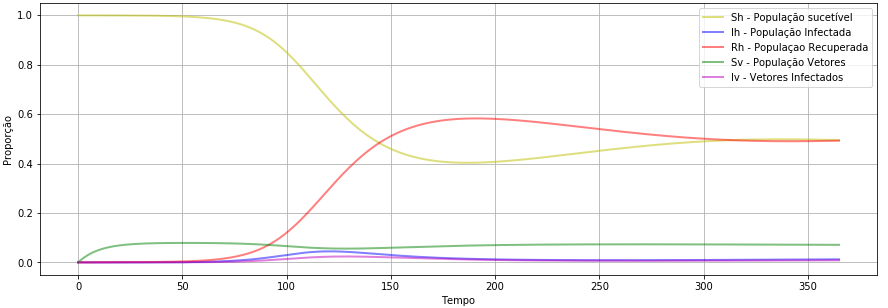
\includegraphics[width=0.46\textwidth]{Graf3.png}
    \label{fig:s3}
\end{figure}

\subsubsection{Simulação 4: A 800 - uv 0.25}

Nesta simulação, figura \ref{fig:s4}, novamente, ao aumentar-se a taxa de mortalidade do vetor, o modelo mostra um pequeno crescimento dos vetores, entretanto, não apresenta interação entre as duas populações, o que possivelmente pode ser justificado (novamente) pela insuficiência  de vetores infectados devido a sua baixa densidade populacional em relação aos seres humanos.
\\

\begin{figure}[!ht]
  \caption{Simulação 4 - Nh 100000 - A 800 - uv 0.25}
  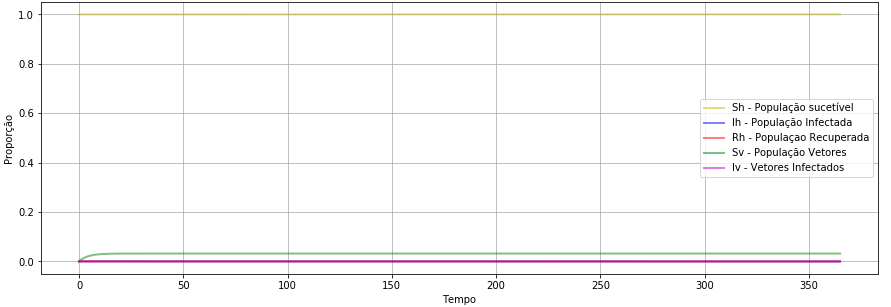
\includegraphics[width=0.46\textwidth]{Graf4.png}
  \label{fig:s4}
\end{figure}

\subsubsection{Simulação 5: A 1600 - uv 0.1}

Nesta simulação, figura \ref{fig:s5}, ao dobrar a taxa com que novos mosquitos aparecem e diminuir a taxa de mortalidade destes, o gráfico apresenta ligeiro crescimento na proporção da população de vetores e consequentemente, um aumento nos seres humanos infectados (tal como vetores). Pode-se observar que agora com este aumento, a proporção da população recuperada aumenta o que possivelmente pode ser justificado pela indicação do início dos contágios.
\\

\begin{figure}[!ht]
  \caption{Simulação 5 - Nh 100000 - A 1600 - uv 0.1}
  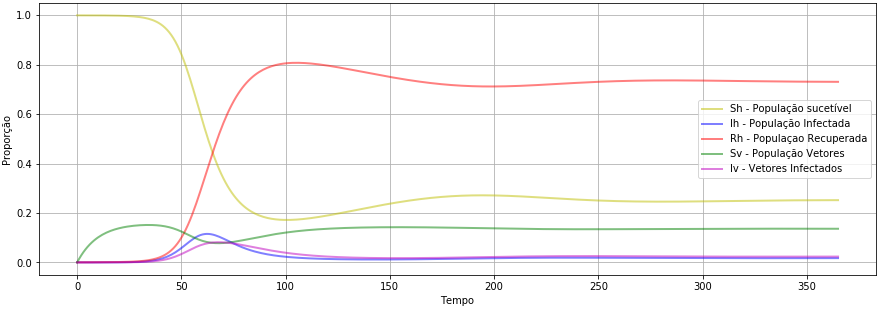
\includegraphics[width=0.46\textwidth]{Graf5.png}
  \label{fig:s5}
\end{figure}

\subsubsection{Simulação 6: A 1600 - uv 0.25}

Nesta simulação, figura \ref{fig:s6} mais uma vez, ao manter a taxa de crescimento dos vetores e aumentar a taxa de mortalidade, há um crescimento na proporção de vetores existentes, porém, nenhuma interação vetor-doença-ser humano é detectada pelo modelo matemático.
\\

\begin{figure}[!ht]
  \caption{Simulação 6 - Nh 100000 - A 1600 - uv 0.25}
  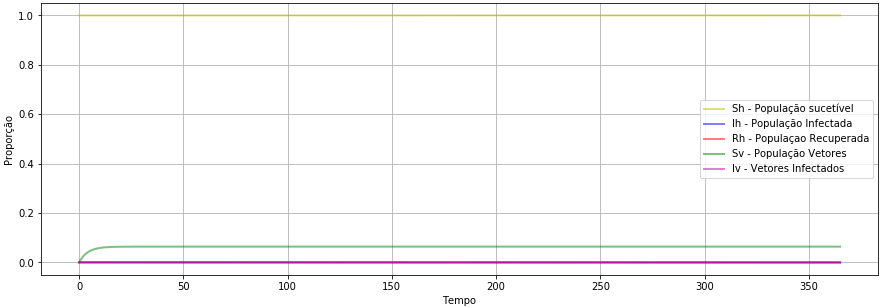
\includegraphics[width=0.46\textwidth]{Graf6.png}
      \label{fig:s6}
\end{figure}

\subsubsection{Simulação 7: A 3200 - uv 0.1}

Nesta simulação, figura  \ref{fig:s7} dobrou-se a taxa de crescimento da população de vetores e diminuiu-se a taxa de mortalidade. Como resposta, em comparação com os ensaios anteriores, as proporções de vetores, vetores infectados tal como humanos infectados aumentaram. Desta vez, nota-se um padrão na proporção de pessoas suscetíveis e pessoas recuperadas, isso pode ser possivelmente explicado pelo fato da Dengue, apesar de existir quatro tipos de vírus, ao contrair Dengue pela primeira vez e se recuperar, a possibilidade de ser contraída novamente diminui, o que é mostrado pela diminuição da população suscetível e aumento da população recuperada.
\\

\begin{figure}[!ht]
  \caption{Simulação 7 - Nh 100000 - A 3200 - uv 0.1}
  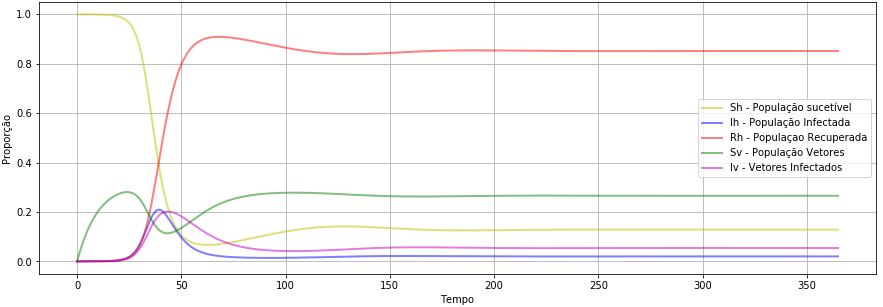
\includegraphics[width=0.46\textwidth]{Graf7.png}
  \label{fig:s7}
\end{figure}

\subsubsection{Simulação 8: A 3200 - uv 0.25}

Nesta simulação, figura  \ref{fig:s8} verificou-se uma aumento taxa de mortalidade. Como resposta o modelo matemático mostrou que com tais parâmetros a população dos vetores se mantém, entretanto não existe uma proporção expressiva de vetores humanos infectados em comparação com o gráfico anterior. 
\\

\begin{figure}[!ht]
  \caption{Simulação 8 - Nh 100000 - A 3200 - uv 0.25}
  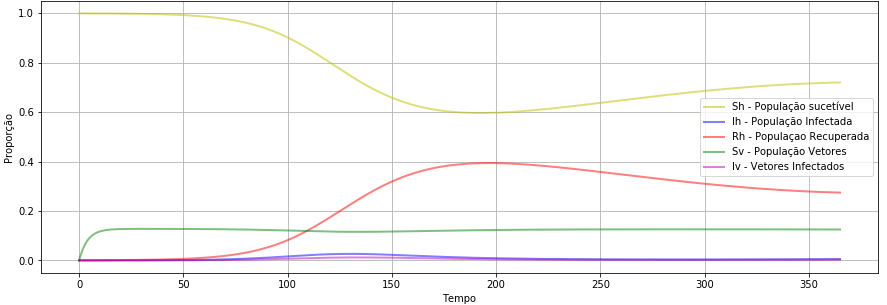
\includegraphics[width=0.46\textwidth]{Graf8.png}
  \label{fig:s8}
\end{figure}

\subsubsection{Simulação 9: A 5.000 - uv 0.1}

Nesta simulação, figura \ref{fig:s9}, aumentou-se a taxa de aparição de vetores e diminuiu-se a taxa de mortalidade. As proporções de existência de vetores, vetores infectados e população infectada tiveram aumentos muito superiores aos ensaios anteriores. Novamente o padrão entre População Suscetível X População Recuperada se faz presente, o que pode ser explicado pelo fato de que ao existir menos pessoas suscetíveis, esta se dá desta forma, pois já foram infectadas.
\\
\begin{figure}[!ht]
  \caption{Simulação 9 - Nh 100000 - A 5.000 - uv 0.1}
  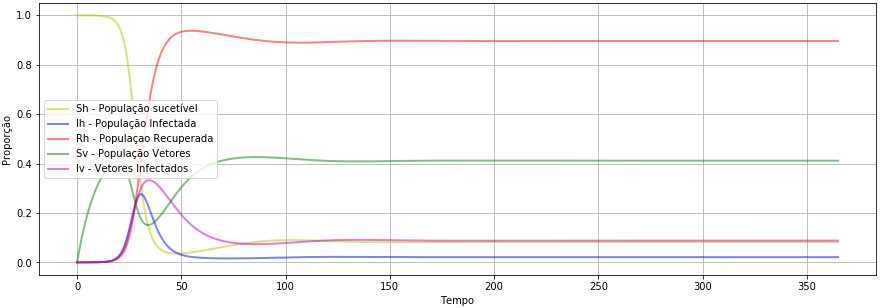
\includegraphics[width=0.46\textwidth]{Graf9.png}
  \label{fig:s9}
\end{figure}


\subsubsection{Simulação 10: A 5000 - uv 0.25}

Nesta simulação, figura \ref{fig:s10}, com o aumento da taxa de mortalidade do vetor, as proporções de infecção diminuem (logicamente viável). Nesta simulação, o padrão entre População Suscetível X População Recuperada apresenta uma ligeira oscilação e em seguida se estabiliza, o que possivelmente pode ser explicado pelo fato das densidades estarem de certa forma “ideais”, isto é, mais próxima de uma versão da realidade, pois há variação tanto de pessoas suscetíveis como recuperadas, devido ao pico na proporção de infecção no início do gráfico.
\\

\begin{figure}[!ht]
  \caption{Simulação 10 - Nh 100000 - A 5000 - uv 0.25}
  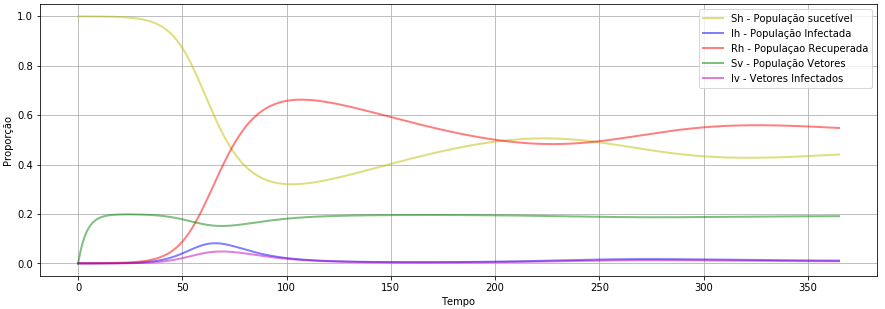
\includegraphics[width=0.46\textwidth]{Graf10.png}
  \label{fig:s10}
\end{figure}

\subsection{Análise Geral}

É válido ressaltar que apenas os parâmetros tal como a variação destes não são exclusivos para a determinação de alguma hipótese, e para isso, outros detalhes sobre outros parâmetros implícitos serão discutidos a seguir\\

\subsubsection{A Dengue pode ser contraída mais de uma vez?}  
 
Segundo \cite{espiritosanto} Ao contrair dengue, a pessoa fica imunizada permanentemente para aquele sorotipo de vírus, mas não para os outros. Dessa forma, uma mesma pessoa pode ter dengue até quatro vezes. A segunda infecção por qualquer sorotipo da dengue é, na maioria das vezes, mais grave do que a primeira, independentemente dos sorotipos e de sua sequência. Contudo, o tipo 3 mostra-se mais virulento. É importante lembrar, porém, que manifestações mais graves da dengue podem ocorrer na primeira infecção\\

O fato de o indivíduo ser imunizado após o contágio pode ser a justificativa para as respostas no gráfico cujo as curvas de pessoas suscetíveis e recuperadas tenham certo padrão.

\subsubsection{População de \textit{Aedes aegypti} em área endêmica de dengue}

Reiterando, a taxa da população de vetores deve ser considerada porém não é a única a ser contemplada. A região e nível socioeconômico também deve se aceitar. Segundo a Revista Saúde Publica\cite{barata2001aedes}, um nível socioeconômico mais baixo e com maior concentração populacional apresentam condições mais favoráveis à proliferação do vetor e, portanto, maior risco de transmissão de dengue.\\

A Figura \ref{fig:regioes} mostra as regiões endêmicas da Dengue:

\begin{figure}[!ht]
  \caption{Regiões endêmicas de Dengue\cite{bohm2016dengue}}
  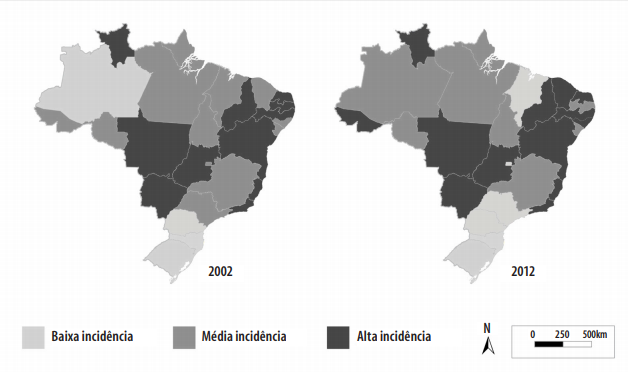
\includegraphics[width=0.46\textwidth]{regiaoendemica.png}
  \label{fig:regioes}
\end{figure}

Pode-se afirmar que a aplicação deste modelo matemático depende da região de estudo, pois o índice de incidência da doença é um fator relevante a se considerar. Uma aplicação na região Centro Oeste do Brasil (que por apresentar um clima mais quente também contribui para a proliferação da doença) certamente irá ser muito mais aproveitada do que na região Sul, onde apresenta baixa incidência.

\subsubsection{Dados da região (Brasil)}

Ademais, informações em relação a cada região no que se diz respeito a natalidade, mortalidade, distribuição da população podem influenciar na análise do modelo. Tais parâmetros podem ser (segundo IBGE): População Total, População por Sexo e grupo de Idade, Distribuição da população (por sexo e idade), Esperanças de vida ao nascer, taxas brutas de mortalidade e natalidade, taxas de fecundidade e proporção de migrantes entre regiões.\\

Abaixo é apresentado um gráfico (IBGE) das taxas brutas de mortalidade do Brasil de 2000 a 2015, dado extremamente relevante que deve ser levado em consideração no momento da aplicação do estudo do modelo matemático.

\begin{figure}[!ht]
  \caption{Taxas brutas de mortalidade do Brasil de 2000 a 2015\cite{ibge-mortalidade}}
  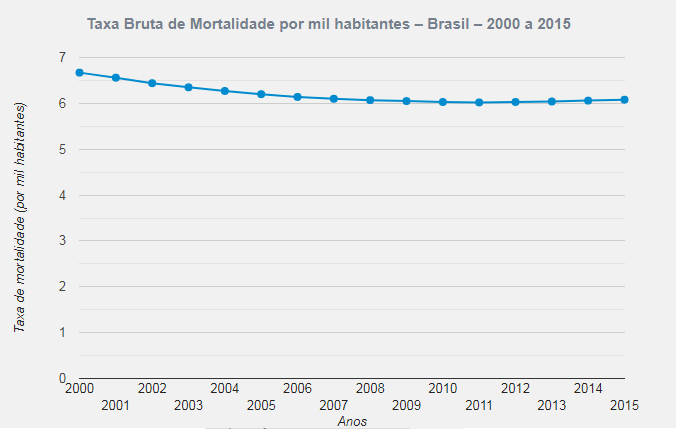
\includegraphics[width=0.46\textwidth]{taxamorte.png}
  \label{fig:taxamorte}
\end{figure}

\subsubsection{Casos registrados}

Uma vez que as taxas de natalidade e mortalidade interferem na aplicação, a situação epidemiológica do país também tem sua parcela de interferência. A tabela abaixo (Ministério da Saúde) apresenta casos prováveis, confirmados, óbitos e descartados de Dengue.
Claramente uma região que não é propícia para a Dengue (ao contrário do Brasil) não terá uma resposta da aplicação do modelo tão satisfatória. A figura \ref{fig:arboviroses} mostra a situação epidemiológica de arboviroses no Brasil

\begin{figure}[!ht]
  \caption{Situação epidemiológica de arboviroses no Brasil\cite{svs}}
  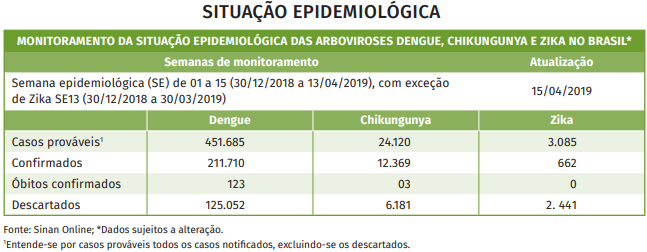
\includegraphics[width=0.46\textwidth]{arboviroses.png}
  \label{fig:arboviroses}
\end{figure}

\subsubsection{Casos registrados (por Estados)}
Para uma aplicação correta do modelo, devem-se levar em conta as informações de cada região. No caso deste trabalho, os dados contemplaram todo o país, mas como caráter informativo, a figura abaixo apresenta os dados referentes a cada estado. Algumas regiões mostram números elevados o que mostra que o estudo de modelos dinâmicos para a dengue no Brasil deve ser implementado para buscar-se melhoria na sociedade.

\begin{figure}[!ht]
  \caption{Casos de Dengue registrados por Estado\cite{svs}}
  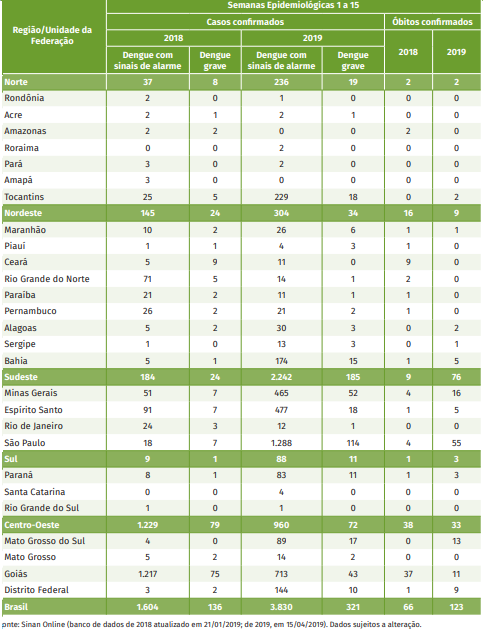
\includegraphics[width=0.46\textwidth]{casos.png}
  \label{fig:casos}
\end{figure}

\subsubsection{Detalhes do modelo matemático utilizado}
No item (x do desenvolvimento que é mostrado os parâmetros do modelo matemático) foi apresentado os parâmetros utilizados
O vetor de condições iniciais usado no modelo se encontra abaixo:

 $$
  y0 = \left[
\begin{array}{rrrrr}
 Sh & Ih & Rh & Sv & Iv
\end{array}\right]
$$

Uma vez que o vetor de condições iniciais é tal que leva em consideração os parâmetros acima, uma mínima alteração em qualquer parâmetro, o estado inicial se altera e consequentemente o modelo apresenta outro comportamento. Como exemplo, o parâmetro ‘b’ é definido como quantas vezes por dia um mosquito pica as pessoas, um dado que é quase subjetivamente dimensionado e pode interferir no estudo.\\

Entretanto, o modelo se mostrou consistente nos ensaios realizados com as diferentes variações de taxas. Não se pode com certeza definir conclusões quantitativas devido às minúcias nos parâmetros utilizados, contudo, é possível chegar a conclusões conceituadas, das quais foram evidentes nos testes executados como:\\

\begin{enumerate}
    \item A taxa de mortalidade do vetor tem maior influencia do que o crescimento deste;
    
    \item Uma vez que o indivíduo contrai Dengue, ele se torna um indivíduo recuperado e menos suscetível a doença, o que é mostrado no padrão da curva de Pessoas Recuperadas X Pessoas Suscetíveis;
    
    \item Uma densidade populacional de vetores baixa não surge efeito algum na população de seres humanos no momento do contágio do vírus. (Situação ideal buscada pela realidade);
    
    \item O sistema de modelo de doenças endêmicas pode ser considerado um sistema dinâmico estável, pois após o período transitório, este se estabiliza.
    
    
    \item Por fim, é possível detectar possíveis surtos da doença através do estudo gráfico e consequentemente  buscar formas de diminuí-lo a fim de proporcionar uma redução das incidências de Dengue com o objetivo de alcançar uma melhor qualidade de vida para aqueles que vivem em regiões endêmicas sujeitos ao contágio da doença.
    
\end{enumerate}

\section{Conclusão}

Consoante aos dados e argumentos apresentados ao longo do desenvolvimento deste trabalho foi possível observar o comportamento do modelo matemático SIR na aplicação de sistemas dinâmicos como o espalhamento de doenças endêmicas. Os seus parâmetros foram adaptados para a realidade brasileira para se estudar os casos de Dengue, o qual se mostrou bem aferido, pois conseguiu prever em sua maior parte o número de casos de anos presentes com dados de anos anteriores. Também foi possível utilizara adaptação do modelo para propagação através de vetores, como o mosquito Aedes Egypt, o que permitiu uma análise mais minuciosa do caso escolhido para análise.

\section*{Agradecimentos}
Agradecemos ao professor Antonio Carlos Zambroni e ao mestrando Pedro Henrique Naves Vasconcelos, nosso muito obrigado pelo conhecimento transmitido, confiança e compreensão. 
% \nocite{*}


\def\BibTeX{BibTeX}
\bibliographystyle{IEEEtran}
\bibliography{IEEEabrv,./references}

\section*{ANEXO I: Algoritmo da Simulação em linguagem Python versão 3.7}

\begin{lstlisting}[language=Python]
#!/usr/bin/env python
# coding: utf-8
import scipy.integrate
import numpy
import matplotlib.pyplot as plt
import itertools

def deriv(y, t, Nh, Bh, gamma, u_h, 
    b, m, A, u_v, Bv):
    
    Sh, Ih, Rh, Sv, Iv = y
    dShdt = ( 
        u_h*(Nh-Sh) - (
            (Bh * b)*(Sh * Iv)/(Nh + m)
        ))
    dIhdt = 
        (Bh * b) * (Sh * Iv)/ (Nh + m)  - (
        (u_h + gamma) * Ih)
    dRhdt = 
        (gamma * Ih) - (u_h * Rh)
    dSvdt = 
        A - (
        (Bv *  b)*(Sv*Ih)/(Nh + m)
        ) - (u_v * Sv)
    dIvdt = (
        (Bv * b)*(Sv*Ih)/(Nh+m)
        ) - (u_v * Iv)
    return dShdt, dIhdt, dRhdt, dSvdt, dIvdt

populacao = [100000]
novos_mosquitos = [
    400, 800, 1600, 3200, 5000]
mortalide_mosquitos = [0.1,  0.25]

dias = [
    45, 40, 45, 35, 365, 35, 45, 35, 
    40, 40, 70, 90, 50, 60, 50,
]

p_escalar = itertools.product(
    populacao, 
    novos_mosquitos, 
    mortalide_mosquitos
)

for idx, (Nh, A, u_v) in enumerate(p_escalar):
    Bh = 0.75
    gamma = 0.25
    u_h = 6 / 1000
    b = 1
    m = 0
    Bv = 1
    Ih = 49.2  
    Rh = 49.2  
    Sv = 0
    Iv = 0
    Sh = Nh - Ih

    t = numpy.linspace(0, 365, 365)
    y0 = Sh, Ih, Rh, Sv, Iv
    args = \
        Nh, Bh, gamma, u_h, b, m, A, u_v, Bv
    ret = scipy.integrate.odeint(
        deriv, y0, t, args=args)
    Sh, Ih, Rh, Sv, Iv = ret.T
    
    plt.figure(figsize=[15,5])
    plt.plot(t, Sh/Nh, 'y', alpha=0.5, 
        lw=2, label='Sh')
    plt.plot(t, Ih/Nh, 'b', alpha=0.5, 
        lw=2, label='Ih')
    plt.plot(t, Rh/Nh, 'r', alpha=0.5, 
        lw=2, label='Rh')
    plt.plot(t, Sv/Nh, 'g', alpha=0.5, 
        lw=2, label='Sv')
    plt.plot(t, Iv/Nh, 'm', alpha=0.5, 
        lw=2, label='Iv')
    plt.grid()
    plt.legend()
    plt.xlabel("Tempo")
    plt.ylabel("Proporcao")
    plt.title(
        "N:{} Nh:{} A:{} uv:{}".format(
            idx+1, Nh, A, u_v))
    plt.show()
\end{lstlisting}

Código completo e outras simulações realizadas consulte \cite{mileo}.


\end{document}
